% Provenance (never printed): old terminale S material on the disappearance of
% mountain ranges (erosion, transport, sedimentation, isostatic rebound, the
% recycling of continental material). Owner (Sync 0/1): denudation rate,
% sediment load (bed, suspended, dissolved), isostatic rebound, detrital rock,
% diagenesis. Weathering, erosion, deposition are Book 1's (g5); hydrolysis and
% clay minerals g10.07's; discharge g10.08's; isostasy and Airy's model g11.03's;
% sedimentary basin g11.09's; mountain root g12.01's; metamorphism g12.03's;
% half-life is physics' (recalled in prose). Figures: figdata/grade-12/relief_decay.py
% (rates, decay curves, the Varden unconformity from figdata/shared/region.py).
\chapter{De afbraak van gebergten}\label{ch:g12:destruction-of-mountains}

Gezien vanuit het Internationaal Ruimtestation vormen de Appalachen in het
oosten van Noord-Amerika een opvallend patroon van lange, donkere, beboste ruggen
en bleke landbouwdalen, meer dan \qty{500}{km} ervan op de foto
hieronder. De ruggen zijn harde gesteentelagen die tot nauwe \omterm{def:g12:mountain-building:fold}{plooien} werden verfrommeld
toen Afrika tegen Noord-Amerika aan drukte, in het Carboon en het
Perm, meer dan 250 miljoen jaar geleden. Vandaag staat hun hoogste top, Mount
Mitchell, het hoogste punt ten oosten van de Mississippi,
\qty{2037}{m} boven zeeniveau, minder dan een kwart van de hoogte van de Everest.
% ledger: photo:g12-appalachians, usgs:alleghanian, usgs:alleghanian-age, ics:base.Triassic, ncparks:mitchell (6684 ft), tht:everest (Book 1 row, 8848.86 m)

\begin{omfigure}
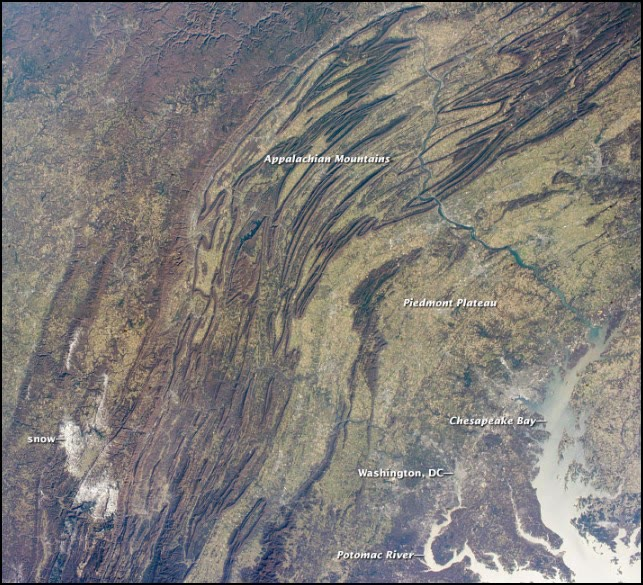
\includegraphics[width=0.6\linewidth]{images/book2/g12-iss-appalachians.jpg}

{\small De Appalachen met hun ruggen en dalen, van het noordoosten van Pennsylvania
(rechtsboven) tot West Virginia, gefotografeerd vanuit het Internationaal
Ruimtestation op 17 november 2012. De beboste ruggen zijn harde gesteentelagen, de
landbouwdalen zachtere. Foto NASA (publiek domein).}
\end{omfigure}
% ledger: photo:g12-appalachians

Een gebergteketen blijft niet bestaan. Vanaf het moment dat ze oprijst, vallen regen, ijs en
rivieren haar aan; het gesteente dat ze wegvoeren, belandt in de zee, waar het
nieuw gesteente wordt. Dit hoofdstuk meet hoe snel dat gaat, volgt het
puin tot de plaats waar het tot steen wordt, en laat zien waarom een keten die
wordt afgesleten, onderweg blijft stijgen.

\begin{recall}
Verwering breekt gesteente af waar het staat; erosie voert het puin weg
en afzetting legt het elders neer (Boek 1, jaar 5). \omterm{def:g10:soil-formation:chemical-weathering}{Chemische verwering}
maakt van veldspaten kleimineralen door \omterm{def:g10:soil-formation:hydrolysis}{hydrolyse}
(\cref{ch:g10:soil-formation}). Het debiet van een rivier is het volume
water dat in een seconde een punt passeert (\cref{ch:g10:drainage-basins}). De
korst drijft in \omterm{def:g11:lithosphere-asthenosphere:isostasy}{isostasie} op de mantel; in het model van Airy staat een gebied waarvan de korst
dikker is met $\Delta H$, hoger met $\Delta H\,(\rho_m - \rho_c)/\rho_m$
(\cref{ch:g11:lithosphere-asthenosphere}), en een hoge keten rust op een \omterm{def:g12:continental-crust:root}{wortel}
van dikke korst (\cref{ch:g12:continental-crust}). Sedimenten hopen zich op in
\omterm{def:g11:fossil-fuel-geology:basin}{sedimentaire bekkens} (\cref{ch:g11:fossil-fuel-geology}). Gesteenten die diep in
een gebergtegordel worden begraven, worden gemetamorfoseerd (\cref{ch:g12:metamorphic-rocks}).
\end{recall}

\section{Hoe snel wordt het land afgesleten?}

\begin{definition}[Denudatiesnelheid]\label{def:g12:destruction-of-mountains:denudation}
De \emph{denudatiesnelheid}\index{denudatiesnelheid} van een gebied is de gemiddelde
dikte gesteente die verwering en erosie samen er per
tijdseenheid van weghalen. Ze wordt meestal gegeven in meter per miljoen jaar
(\unit{m/Myr}), wat hetzelfde is als millimeter per duizend jaar.
\end{definition}
% ledger: pb11:rates (rates in m/Myr), earle:loads

Hoe meet je iets dat zo traag gaat? Kosmische straling die de grond treft, maakt
een zeldzame isotoop, beryllium-10, in het kwarts van de bovenste paar meter gesteente.
Hoe trager een oppervlak wordt afgesleten, hoe langer elke korrel dicht bij de top blijft,
en hoe meer beryllium-10 hij verzamelt. Wie het meet in het zand van een rivier,
krijgt de gemiddelde \omterm{def:g12:destruction-of-mountains:denudation}{denudatiesnelheid} van het hele \omterm{def:g10:drainage-basins:drainage-basin}{stroomgebied} stroomopwaarts, over de laatste
duizenden tot miljoenen jaren.
% ledger: pb11:rates (10Be produced within a few metres of the surface; concentration reflects near-surface residence time; 10^3 to 10^6 years)

Een overzicht van 1599 zulke metingen vond dat kale rotsontsluitingen
traag worden afgesleten, gemiddeld met \qty{12}{m/Myr} (mediaan
\qty{5.4}{m/Myr}), en nooit sneller dan met \qty{140}{m/Myr}. Hele
\omterm{def:g10:drainage-basins:drainage-basin}{stroomgebieden} verliezen veel meer, gemiddeld \qty{218}{m/Myr}, maar met een mediaan van
maar \qty{54}{m/Myr}: een paar snelle \omterm{def:g10:drainage-basins:drainage-basin}{stroomgebieden} trekken het gemiddelde omhoog. De snelste zijn
de steile: de gemiddelde helling van een \omterm{def:g10:drainage-basins:drainage-basin}{stroomgebied} is de factor die zijn snelheid
het best voorspelt. \omterm{def:g10:drainage-basins:drainage-basin}{Stroomgebieden} in seismisch actieve gebieden, waar gebergten stijgen,
eroderen ongeveer twee keer zo snel als die in rustige gebieden.
% ledger: pb11:rates

\begin{omfigure}
\begin{tikzpicture}
\begin{axis}[omrecord, xbar, xmode=log, log origin=infty, bar width=7pt, bar shift=0pt,
  width=0.62\linewidth, height=6.6cm, scale only axis, xmin=3, xmax=1000,
  ymin=0.4, ymax=10.6, ytick={1,...,10}, y tick label style={font=\scriptsize, align=right},
  yticklabels={{ontsluitingen, mediaan}, {ontsluitingen, gemiddelde}, {rivieren wereld (balans)}, {stroomgebieden, mediaan},
    {Mississippi, vóór 1900 (balans)}, {droge stroomgebieden, gem.}, {rustige stroomgebieden, gem.}, {stroomgebieden, gem.},
    {seismisch actieve stroomgebieden, gem.}, {poolstroomgebieden, gem.}},
  xlabel={denudatiesnelheid (\unit{m/Myr}), logaritmische schaal}, ymajorgrids=false,
  unbounded coords=discard, nodes near coords, nodes near coords align={horizontal}, nodes near coords style={font=\scriptsize},
  point meta=rawx, every node near coord/.append style={/pgf/number format/.cd, fixed, precision=0}]
% computed in figdata/grade-12/relief_decay.py; ledger: pb11:rates, mm10:mississippi, kammerer:mississippi, earle:loads, cm95:crust
\addplot[fill=omThm!45, draw=omThm, every node near coord/.append style={/pgf/number format/.cd, fixed, precision=1}] table[x=measured, y=idx] {figdata/out/grade-12-relief_decay-rates.dat};
\addplot[fill=omDef!45, draw=omDef] table[x=budget, y=idx] {figdata/out/grade-12-relief_decay-rates.dat};
\end{axis}
\end{tikzpicture}

{\small Denudatiesnelheden gemeten met beryllium-10 (rood: 1599 metingen,
waarvan 1149 in rivierzand) en twee snelheden die in dit hoofdstuk zijn berekend uit het
sediment dat rivieren meevoeren (blauw); gem.\ = gemiddelde. Bronnen: Portenga en Bierman (2011);
Meade en Moody (2010); Syvitski en anderen (2005).}
\end{omfigure}
% values: world_m_per_myr 43.5, miss_before_1900_m_per_myr 55.8 (relief_decay.py)

\section{Rivieren voeren de gebergten weg}

Veel van wat van het land wordt afgesleten, verlaat het via rivieren.

\begin{definition}[Sedimentvracht]\label{def:g12:destruction-of-mountains:load}
De \emph{sedimentvracht}\index{sedimentvracht} van een rivier is het materiaal dat ze
meevoert, in drie vormen: de \emph{bodemvracht}\index{bodemvracht}, grote korrels
die over de bodem worden gerold, geduwd of gestuiterd; de \emph{zwevende
vracht}\index{zwevende vracht}, kleine korrels die in het stromende water zweven; en
de \emph{opgeloste vracht}\index{opgeloste vracht}, ionen in oplossing, zoals
calcium en chloride, achtergelaten door \omterm{def:g10:soil-formation:chemical-weathering}{chemische verwering}.
\end{definition}
% ledger: earle:loads

Gemiddeld is de \omterm{def:g12:destruction-of-mountains:load}{opgeloste vracht} ongeveer \qty{15}{\percent} van de massa die een
rivier meevoert. Hoe sneller het water, hoe grotere korrels het kan optillen. Een
zandkorrel van \qty{1}{mm} wordt van de bodem opgepakt bij ongeveer
\qty{20}{cm/s}, en eenmaal in beweging blijft hij zweven tot de stroming
onder \qty{10}{cm/s} zakt. Siltkorrels zijn moeilijker op te tillen dan zand,
omdat ze aan elkaar kleven: een korrel van \qty{0.01}{mm} heeft
\qty{60}{cm/s} nodig om te worden opgepakt, maar daarna houdt een stroming van \qty{0.1}{cm/s} hem
zwevend. Daarom stromen rivieren bij hoogwater bruin, en daarom
reist de fijnste modder helemaal tot in zee.
% ledger: earle:loads

\begin{omfigure}
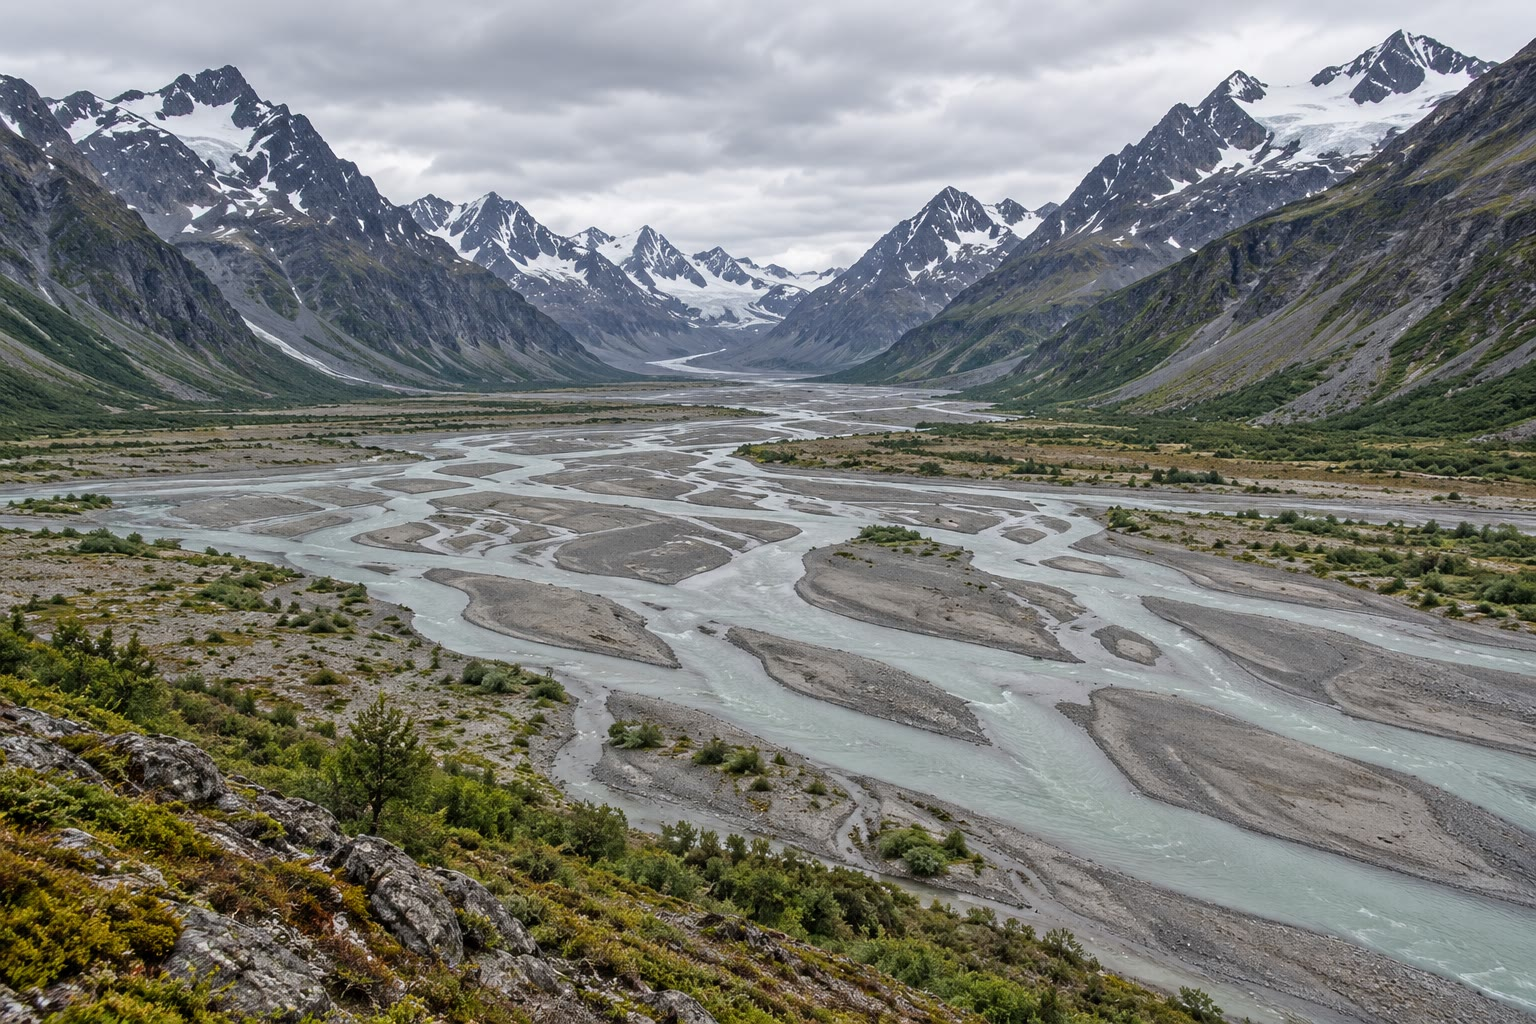
\includegraphics[width=0.66\linewidth]{images/book2/ai/g12-braided-river.jpg}

{\small Een vlechtende rivier in een gletsjerdal in het gebergte: ondiepe geulen splitsen
zich en komen weer samen tussen grindbanken die het water alleen bij hoogwater verplaatst.
AI-illustratie.}
\end{omfigure}

Meten wat een rivier meevoert, geeft een tweede manier om een \omterm{def:g12:destruction-of-mountains:denudation}{denudatiesnelheid} te vinden.

\begin{method}[Een erosiebalans]\label{met:g12:destruction-of-mountains:budget}
\begin{enumerate}
  \item Neem de massa sediment die de rivier in een jaar meevoert, en tel de
        \omterm{def:g12:destruction-of-mountains:load}{opgeloste vracht} erbij op (als alleen de vaste vracht bekend is, deel die dan door
        $0.85$).
  \item Deel door de dichtheid van het gesteente, ongeveer \qty{2830}{kg/m^3} voor de
        \omterm{def:g12:continental-crust:continental-crust}{continentale korst}, om het volume gesteente te krijgen dat elk jaar wordt weggehaald.
  \item Deel door de oppervlakte van het \omterm{def:g10:drainage-basins:drainage-basin}{stroomgebied}: dit is de dikte die
        elk jaar wordt weggehaald.
  \item Vermenigvuldig met $10^6$ om haar uit te drukken in meter per miljoen jaar.
\end{enumerate}
\end{method}
% ledger: earle:loads, cm95:crust

\begin{example}[De Mississippi]\label{ex:g12:destruction-of-mountains:mississippi}
Vóór 1900 voerde het riviersysteem van de Missouri en de Mississippi ongeveer 400
miljoen ton sediment per jaar naar zee, uit een \omterm{def:g10:drainage-basins:drainage-basin}{stroomgebied} van ongeveer
\qty{2980000}{km^2}. Met de \omterm{def:g12:destruction-of-mountains:load}{opgeloste vracht} is dat $400/0.85 \approx 471$ miljoen
ton, dat is $\num{4.71e11}/2830 \approx \qty{1.66e8}{m^3}$ gesteente per jaar.
Uitgespreid over $\qty{2.98e12}{m^2}$ is het een laag van
\[
  \frac{\num{1.66e8}}{\num{2.98e12}} \approx \qty{5.6e-5}{m}
  \text{ per jaar, ongeveer } \qty{56}{m/Myr}.
\]
Tussen 1987 en 2006 voerde de rivier maar 145 miljoen ton per jaar mee, wat
ongeveer \qty{20}{m/Myr} geeft: dammen die in de jaren 1950 op de Missouri zijn gebouwd, houden
ongeveer 100 tot 150 miljoen ton per jaar vast, en andere werken houden er nog meer tegen.
\end{example}
% ledger: mm10:mississippi, kammerer:mississippi, earle:loads, cm95:crust
% values: miss_before_1900_m_per_myr 55.8, miss_1987_2006_m_per_myr 20.2 (relief_decay.py)

Dezelfde balans kan voor de hele wereld worden opgesteld. Voordat mensen de
rivieren veranderden, voerden die ongeveer 15.5 miljard ton vast sediment per jaar naar
de kusten; met de \omterm{def:g12:destruction-of-mountains:load}{opgeloste vracht} is dat ongeveer \qty{6.4}{km^3} gesteente per
jaar, weggenomen van de \qty{1.48e8}{km^2} van de continenten: een gemiddelde
\omterm{def:g12:destruction-of-mountains:denudation}{denudatiesnelheid} van ongeveer \qty{43}{m/Myr}, dicht bij de mediaan van de beryllium-10-metingen.
Mensen hebben sindsdien beide termen veranderd: bodemerosie heeft
wat rivieren oppikken met ongeveer 2.3 miljard ton per jaar doen toenemen, maar meer
dan 100 miljard ton sediment ligt nu achter dammen.
% ledger: syvitski:modern-flux (Book 1 row, prehuman 15.5 Gt/yr with bed load), sy05:humans, data:etopo1 (land fraction 0.290, grade-11 hypsometry), cm95:crust
% values: world_volume_km3_per_yr 6.44, land_area_km2 1.48e8, world_m_per_myr 43.5 (relief_decay.py)

\section{Van sediment tot gesteente}

Wat de rivieren meevoeren, wordt afgezet waar de stroming vertraagt: in dalen en
meren, op delta's, en vooral in de \omterm{def:g11:fossil-fuel-geology:basin}{sedimentaire bekkens} van de continentale
randen. Laag na laag wordt het sediment begraven, en langzaam wordt het
gesteente.

\begin{definition}[Detritisch gesteente; diagenese]\label{def:g12:destruction-of-mountains:diagenesis}
Een \emph{detritisch gesteente}\index{detritisch gesteente} (of klastisch gesteente) is een
sedimentair gesteente dat bestaat uit brokstukken, de klasten, van oudere gesteenten en mineralen.
\emph{Diagenese}\index{diagenese} is het geheel van veranderingen die een begraven
sediment bij lage temperatuur tot gesteente maken: \emph{compactie}, wanneer het gewicht van
de lagen erboven water en lucht eruit perst, en daarna \emph{cementatie}, wanneer
mineralen die uit het water in de poriën kristalliseren (calciet, kwarts,
hematiet, kleimineralen) de korrels aan elkaar kitten.
\end{definition}
% ledger: earle:clastic

Detritische gesteenten worden benoemd naar de grootte van hun klasten:
\begin{itemize}
  \item een \textbf{conglomeraat} bestaat uit afgeronde klasten groter dan
        \qty{2}{mm}, een \textbf{breccie} uit hoekige;
  \item een \textbf{zandsteen} bestaat uit zand, korrels tussen \qty{2}{mm}
        en \qty{0.063}{mm}, meestal van kwarts, het mineraal dat het best
        tegen verwering bestand is;
  \item een \textbf{slibgesteente} bevat minstens \qty{75}{\percent} silt en klei;
        het is een schalie als het in dunne lagen splijt.
\end{itemize}
% ledger: earle:clastic

\begin{omfigure}
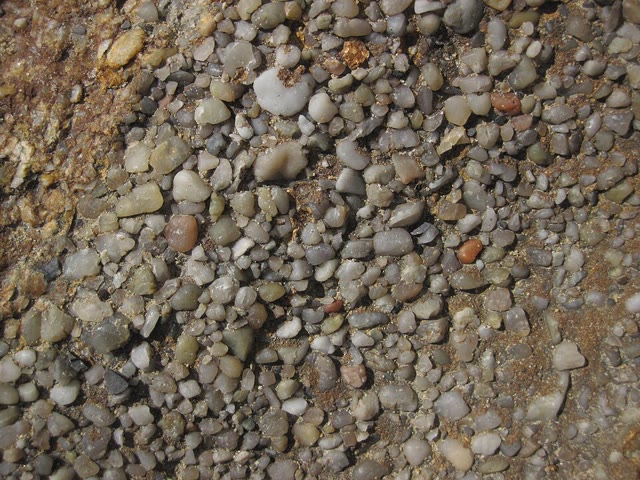
\includegraphics[width=0.5\linewidth]{images/book2/g12-stjohn-conglomerate.jpg}

{\small Een conglomeraat met kwartskeien uit Ohio, uit het Carboon:
afgeronde kiezels van kwarts, gecementeerd door fijner zand. Foto James
St.~John (CC~BY~2.0).}
\end{omfigure}
% ledger: photo:g12-conglomerate, ics:base.Carboniferous, ics:base.Permian (Lower Pennsylvanian lies in the Carboniferous)

De klasten leggen de reis vast. Afgeronde kiezels hebben ver gerold in een
rivier of op een strand; hoekige hebben nauwelijks gereisd. Een zandsteen die
bijna alleen uit kwarts bestaat, komt van gesteente dat lang is verweerd,
tot de andere mineralen klei waren geworden.
% ledger: earle:clastic (rounded/angular, most sand grains quartz, the most resistant mineral)

\section{De wortel stijgt}

Als erosie gewoon gesteente van de top van een keten weghaalde, zou een keten van \qty{2}{km}
hoog, afgesleten met \qty{200}{m/Myr}, in tien miljoen jaar verdwenen zijn.
Maar de keten drijft op de mantel. Terwijl er gesteente van de top wordt weggehaald, wordt de
kolom lichter, en ze stijgt.

\begin{definition}[Isostatisch herstel]\label{def:g12:destruction-of-mountains:rebound}
\emph{Isostatisch herstel}\index{isostatisch herstel} is het stijgen van een gebied van
de \omterm{def:g11:lithosphere-asthenosphere:lithosphere}{lithosfeer} wanneer er een last van wordt weggenomen --- gesteente dat door erosie is afgesleten,
of een ijskap die smelt --- tot de \omterm{def:g11:lithosphere-asthenosphere:isostasy}{isostasie} hersteld is.
\end{definition}
% ledger: sella07:gia (rebound after ice unloading)

\begin{proposition}[Erosie en herstel]\label{prop:g12:destruction-of-mountains:rebound}
Wanneer erosie in het model van Airy een dikte $e$ korst met dichtheid
$\rho_c$ weghaalt van een gebied in \omterm{def:g11:lithosphere-asthenosphere:isostasy}{isostasie} op een mantel met dichtheid $\rho_m$, zakt het
oppervlak maar met
\[
  \Delta h = e\left(1 - \frac{\rho_c}{\rho_m}\right),
\]
terwijl de basis van de korst met $e\,\rho_c/\rho_m$ stijgt.
\end{proposition}

\begin{proof}
Wie $e$ van de top weghaalt, maakt de korst $e$ dunner. Volgens het model van Airy
staat een korst die $e$ dunner is, lager met $e\,(\rho_m - \rho_c)/\rho_m = e(1 -
\rho_c/\rho_m)$. De top van de korst is met dit bedrag gezakt, en haar
dikte is met $e$ afgenomen, dus is haar basis gestegen met $e - e(1 -
\rho_c/\rho_m) = e\,\rho_c/\rho_m$.
\end{proof}

Met $\rho_c = \qty{2830}{kg/m^3}$ en $\rho_m = \qty{3380}{kg/m^3}$ is $1 -
\rho_c/\rho_m \approx 0.163$. Wie \qty{1}{km} gesteente weghaalt, laat het
oppervlak maar ongeveer \qty{163}{m} zakken: de andere \qty{837}{m} worden goedgemaakt doordat de
hele kolom stijgt. Om een keten \qty{2000}{m} te verlagen, moet erosie
ongeveer $2000/0.163 \approx \qty{12300}{m}$ gesteente weghalen. Gesteenten die meer dan
\qty{12}{km} diep lagen, metamorfe gesteenten en granieten die in de diepte van de
keten zijn ontstaan, bereiken het oppervlak: daarom tonen de oude, afgesleten gebergtegordels
schisten, gneisen en granieten over enorme oppervlakten.
% ledger: cm95:crust, data:prem (rho 3.38 below the Moho)
% values: rebound_fraction 0.16272, lowering_per_km_m 162.7, root_rise_per_km_m 837.3, eroded_for_2000m_km 12.29 (relief_decay.py)

\begin{omfigure}
\begin{tikzpicture}[x=1cm, y=1cm, font=\scriptsize]
  % three columns: before, after erosion without rebound, after rebound
  \foreach \i/\top/\base/\lab in {0/3.0/-3.2/{een keten in isostasie}, 1/2.0/-3.2/{erosie haalt $e$ weg}, 2/2.84/-2.36/{de kolom stijgt}} {
    \begin{scope}[xshift=\i*4.6cm]
      \fill[omLithPeridotite!45] (0,-3.6) rectangle (3.4,-0.6);
      \fill[omLithGranite!55, draw=black!60] (0.5,\base) -- (0.5,0) -- (1.0,\top) -- (2.4,\top) -- (2.9,0) -- (2.9,\base) -- cycle;
      \fill[omLithGranite!55, draw=black!60] (0,0) rectangle (0.5,-0.6);
      \fill[omLithGranite!55, draw=black!60] (2.9,0) rectangle (3.4,-0.6);
      \draw[black!40, densely dashed] (-0.1,0) -- (3.5,0);
      \node[anchor=north, align=center, text width=3.4cm] at (1.7,-3.75) {\lab};
    \end{scope}
  }
  % eroded slab, middle panel
  \draw[omThm, densely dashed] (4.6+1.0,3.0) -- (4.6+2.4,3.0);
  \draw[omThm, |-|] (4.6+2.65,3.0) -- node[right] {$e$} (4.6+2.65,2.0);
  % right panel: the old top and base
  \draw[omThm, densely dashed] (9.2+1.0,3.0) -- (9.2+2.4,3.0);
  \draw[omThm, densely dashed] (9.2+0.5,-3.2) -- (9.2+2.9,-3.2);
  \draw[-{Stealth}, omDef, line width=0.9pt] (9.2+1.7,-3.15) -- (9.2+1.7,-2.45);
  \node[omDef, anchor=west] at (9.2+3.0,-2.8) {wortel stijgt};
  \node[anchor=west] at (9.2+3.0,2.95) {oppervlak lager met};
  \node[anchor=west] at (9.2+3.0,2.55) {maar $0.16\,e$};
  \draw[black!60, |-|] (9.2+2.65,3.0) -- (9.2+2.65,2.84);
  % labels
  \node[anchor=west] at (3.45,-2.1) {mantel};
  \node at (1.7,-1.5) {korst};
\end{tikzpicture}

{\small Erosie en \omterm{def:g12:destruction-of-mountains:rebound}{isostatisch herstel} (schematisch, hoogten niet op schaal). Links:
een keten in \omterm{def:g11:lithosphere-asthenosphere:isostasy}{isostasie}, met haar \omterm{def:g12:continental-crust:root}{wortel}. Midden: erosie haalt een dikte $e$
van de top weg. Rechts: de lichtere kolom stijgt tot de \omterm{def:g11:lithosphere-asthenosphere:isostasy}{isostasie} hersteld is; het
oppervlak eindigt maar $0.163\,e$ lager dan bij het begin, en de \omterm{def:g12:continental-crust:root}{wortel} is
$0.837\,e$ gestegen.}
\end{omfigure}

Hetzelfde herstel is vandaag te zien waar een last snel verdween. De
ijskap die bij het laatste glaciale maximum een groot deel van Canada bedekte, was
het dikst rond de Hudsonbaai. Dat ijs is gesmolten, en het land daar stijgt nog altijd:
met ongeveer \qty{10}{mm} per jaar, zoals gemeten met gps, dat is
\qty{10000}{m/Myr}, ongeveer vijftig keer de gemiddelde \omterm{def:g12:destruction-of-mountains:denudation}{denudatiesnelheid} van
\omterm{def:g10:drainage-basins:drainage-basin}{stroomgebieden}. Verder naar het zuiden,
voorbij de Grote Meren, zakt het land met 1 tot \qty{2}{mm} per jaar.
% ledger: sella07:gia, pb11:rates

\section{Hoe lang blijft een keten bestaan?}

Hoe steiler een \omterm{def:g10:drainage-basins:drainage-basin}{stroomgebied}, hoe sneller het erodeert; voor grote \omterm{def:g10:drainage-basins:drainage-basin}{stroomgebieden} is de
\omterm{def:g12:destruction-of-mountains:denudation}{denudatiesnelheid} evenredig gebleken met hun gemiddelde reliëf. Laten we het
eenvoudigste model nemen dat dat zegt.

\begin{proposition}[Het exponentiële verval van een keten]\label{prop:g12:destruction-of-mountains:decay}
Laat $h(t)$ de gemiddelde hoogte zijn van een keten boven de vlakten eromheen. Als
de \omterm{def:g12:destruction-of-mountains:denudation}{denudatiesnelheid} $E = k\,h$ is, met $k$ een constante, en als de \omterm{def:g11:lithosphere-asthenosphere:isostasy}{isostasie}
voortdurend wordt hersteld, dan geldt
\[
  h(t) = h_0\, e^{-f k t}, \qquad f = 1 - \frac{\rho_c}{\rho_m},
\]
waarbij $h_0$ de hoogte op $t = 0$ is. De hoogte wordt gedeeld door $e$
na elke $\tau = 1/(fk)$, en door twee na elke $\tau \ln 2$.
\end{proposition}

\begin{proof}
In een korte tijd $\mathrm{d}t$ haalt erosie een dikte $E\,\mathrm{d}t
= k h\,\mathrm{d}t$ weg, en volgens de vorige propositie zakt het oppervlak
met $f k h\,\mathrm{d}t$. Dus $h' = -fk\,h$, en de oplossingen van deze
vergelijking zijn $h(t) = h_0\,e^{-fkt}$. Op $t = \tau$ is $h = h_0/e$; $h = h_0/2$
wanneer $fkt = \ln 2$.
\end{proof}

Metingen aan grote \omterm{def:g10:drainage-basins:drainage-basin}{stroomgebieden} geven $k$: zonder enige opheffing zou hun reliëf
in ongeveer 11 miljoen jaar tot een tiende dalen. Dus $e^{-11k} = 0.1$, en $k =
\ln 10/11 \approx 0.209$ per miljoen jaar. Zonder herstel ($f = 1$) zou de
tijdconstante $1/k \approx 4.8$ miljoen jaar zijn. Met herstel is $f
\approx 0.163$ en
\[
  \tau = \frac{1}{0.163 \times 0.209} \approx 29 \text{ miljoen jaar},
\]
en de gemiddelde hoogte halveert elke $29 \ln 2 \approx 20$ miljoen jaar:
door het herstel blijft een keten ongeveer zes keer langer bestaan.
% ledger: ahnert70:decay, cm95:crust, data:prem
% values: k_per_myr 0.20933, tau_none_myr 4.777, tau_rebound_myr 29.36, half_rebound_myr 20.35, half_none_myr 3.31 (relief_decay.py)

\begin{omfigure}
\begin{tikzpicture}
\begin{axis}[omrecord, width=0.7\linewidth, height=5.4cm, xmin=0, xmax=100, ymin=0, ymax=2100,
  xlabel={tijd (miljoen jaar)}, ylabel={gemiddelde hoogte (\unit{m})},
  xtick={0,20,...,100}, ytick={0,500,...,2000}]
% computed in figdata/grade-12/relief_decay.py; ledger: ahnert70:decay, cm95:crust, data:prem
\addplot[omProp, line width=1.1pt, densely dashed] table[x=t_Myr, y=h_none] {figdata/out/grade-12-relief_decay-curve.dat};
\addplot[omDef, line width=1.1pt] table[x=t_Myr, y=h_rebound] {figdata/out/grade-12-relief_decay-curve.dat};
\draw[black!45, densely dotted] (axis cs:20.35,0) -- (axis cs:20.35,1000) -- (axis cs:0,1000);
\draw[omProp, line width=0.4pt] (axis cs:9,304) -- (axis cs:33,215);
\coordinate (none) at (axis cs:33.5,215);
\coordinate (reb) at (axis cs:45,780);
\end{axis}
\node[font=\scriptsize, text=omProp, anchor=west] at (none) {zonder herstel};
\node[font=\scriptsize, text=omDef, anchor=south west] at (reb) {met herstel};
\end{tikzpicture}

{\small De gemiddelde hoogte van een keten van \qty{2000}{m} hoog, afgesleten met een snelheid
die evenredig is met haar hoogte, met en zonder \omterm{def:g12:destruction-of-mountains:rebound}{isostatisch herstel}; met
herstel is na 20 miljoen jaar de helft van de hoogte over (stippellijn).
Snelheidsconstante uit Ahnert (1970); dichtheden van de korst en van de mantel onder
de \omterm{def:g11:seismic-structure:moho}{Moho}.}
\end{omfigure}

De Appalachen stellen dit beeld op de proef. Hun botsing eindigde in het Perm,
meer dan 250 miljoen jaar geleden. Dat is meer dan twaalf keer de tijd die het
model nodig heeft om de hoogte te halveren: $2000 \times e^{-250/29} \approx
\qty{0.4}{m}$. Toch rijst Mount Mitchell nog \qty{2037}{m} boven de zee uit.
Het model alleen kan het huidige reliëf niet verklaren: het gebied moet sindsdien
opnieuw zijn opgeheven, of trager zijn geërodeerd dan het model aanneemt.
% ledger: usgs:alleghanian, usgs:alleghanian-age, ics:base.Triassic, ncparks:mitchell, ahnert70:decay
% values: h_after_250myr_rebound_m 0.40 (relief_decay.py)

Zo worden gebergten gerecycled. Het gesteente dat van een keten is afgesleten, belandt in \omterm{def:g11:fossil-fuel-geology:basin}{sedimentaire
bekkens}, waar het \omterm{def:g12:destruction-of-mountains:diagenesis}{detritisch gesteente} wordt; een deel van dat gesteente wordt diep genoeg
begraven om te worden gemetamorfoseerd of zelfs te smelten, een deel wordt bij een \omterm{def:g11:subduction-zones:subduction}{subductiezone}
naar de mantel afgevoerd (\cref{ch:g12:subduction-magmatism}), en een deel wordt
opnieuw opgeplooid tot een nieuwe keten wanneer twee continenten botsen.
% ledger: ss09:balance (sediment subducted), earle:collision (sediments of both margins in the mountains)

\begin{omfigure}
\begin{tikzpicture}
\begin{axis}[omsection, x=1.25cm, y=0.003125cm, xmin=0, xmax=9.49, ymin=-700, ymax=650,
  xlabel={afstand vanaf A (\unit{km})}, ylabel={hoogte (\unit{m})},
  ytick={-600,-300,0,300,600}, tick label style={font=\scriptsize}, unbounded coords=jump]
% shared region tables (figdata/shared/region.py); unconformity from figdata/grade-12/relief_decay.py; ledger: region:name
\addplot[fill=black!8, draw=black!50, line width=0.3pt, even odd rule] table {figdata/out/shared-region-section-unit-schist.dat};
\addplot[fill=icsTriassic!20, draw=black!50, line width=0.3pt, even odd rule] table {figdata/out/shared-region-section-unit-sandstone.dat};
\addplot[fill=icsJurassic!25, draw=black!50, line width=0.3pt, even odd rule] table {figdata/out/shared-region-section-unit-limestone.dat};
\addplot[fill=icsJurassic!8, draw=black!50, line width=0.3pt, even odd rule] table {figdata/out/shared-region-section-unit-shale.dat};
\addplot[fill=icsCretaceous!20, draw=black!50, line width=0.3pt, even odd rule] table {figdata/out/shared-region-section-unit-chalk.dat};
\addplot[fill=omLithAlluv, draw=black!50, line width=0.3pt, even odd rule] table {figdata/out/shared-region-section-unit-alluvium.dat};
\addplot[black, line width=0.7pt] table {figdata/out/shared-region-section-ground.dat};
\addplot[omThm, line width=1.4pt] table[x=s_km, y=z_m] {figdata/out/grade-12-relief_decay-unconformity.dat};
\addplot[fault] table {figdata/out/shared-region-section-fault.dat};
\node[anchor=south east, font=\small\bfseries] at (axis cs:0,650) {A};
\node[anchor=south west, font=\small\bfseries] at (axis cs:9.49,650) {B};
\node[font=\scriptsize, fill=white, inner sep=1pt] at (axis cs:1.2,-520) {schist, ongeveer 480 Ma};
\coordinate (unc) at (axis cs:1.6,-300);
\end{axis}
\node[font=\scriptsize, text=omThm, anchor=west, fill=white, inner sep=1pt] at ([xshift=4pt]unc) {de discordantie};
\end{tikzpicture}

\smallskip
{\small\tikz\fill[black!8, draw=black!50] (0,0) rectangle (0.35,0.22);~schist \quad
\tikz\fill[icsTriassic!20, draw=black!50] (0,0) rectangle (0.35,0.22);~zandsteen (Trias) \quad
\tikz\fill[icsJurassic!25, draw=black!50] (0,0) rectangle (0.35,0.22);~kalksteen \quad
\tikz\fill[icsJurassic!8, draw=black!50] (0,0) rectangle (0.35,0.22);~schalie \quad
\tikz\fill[icsCretaceous!20, draw=black!50] (0,0) rectangle (0.35,0.22);~krijt \quad
\omve{2.5}}

{\small Doorsnede A--B door de Varden Hills, met de discordantie in rood:
het vlakke grondvlak waarop de zandsteen uit het Trias over de sokkel van schist
werd afgezet, later geplooid en gebroken. Gegevens: het model van de reeks voor de streek.}
\end{omfigure}
% values: unconformity sampled from region.contact_elevation('sandstone'); varden_gap_myr 58.1 (relief_decay.py)

De Varden Hills bewaren het verslag van zo'n cyclus. Hun sokkel is een schist,
ongeveer 480 miljoen jaar geleden gemetamorfoseerd, waarin ongeveer 310 miljoen jaar geleden een graniet
binnendrong --- beide ontstaan kilometers onder het oppervlak van
een oude gebergtegordel. Toch rust de zandsteen uit het Trias, afgezet vanaf ongeveer 252
miljoen jaar geleden, er rechtstreeks op, over een vlak oppervlak: de
discordantie. In minder dan 60 miljoen jaar was dat oude gebergte afgesleten
tot een vlakte en waren zijn diepe gesteenten aan het oppervlak gebracht. De zee
breidde zich daarna over de vlakte uit en begroef haar.
% ledger: region:name (model: schist 480 Ma, granite 310 Ma, erosion, unconformity, Triassic cover), ics:base.Triassic
% values: varden_gap_myr 58.1 (relief_decay.py)

\section{Oefeningen}

\begin{exercise}[$\star$]\label{exo:g12:destruction-of-mountains:1}
Geef het woord: (a) de gemiddelde dikte gesteente die per tijdseenheid van een gebied wordt
weggehaald; (b) de korrels die een rivier over haar bedding rolt en laat stuiteren; (c) de
ionen die een rivier in oplossing meevoert; (d) de veranderingen die een begraven sediment
tot gesteente maken; (e) het stijgen van de \omterm{def:g11:lithosphere-asthenosphere:lithosphere}{lithosfeer} wanneer er een last van wordt weggenomen.
\end{exercise}

\begin{exercise}[$\star$]\label{exo:g12:destruction-of-mountains:2}
Noem het detritische gesteente: (1) afgeronde kiezels van \qtyrange{5}{20}{mm}
die aan elkaar zijn gecementeerd; (2) kwartskorrels van \qty{0.3}{mm}; (3) een gesteente dat
voor \qty{90}{\percent} uit silt en klei bestaat en in dunne platen splijt; (4) hoekige
brokstukken van \qty{3}{cm}.
\end{exercise}

\begin{exercise}[$\star$]\label{exo:g12:destruction-of-mountains:3}
Reken om naar millimeter per jaar: (1) \qty{54}{m/Myr}; (2) \qty{218}{m/Myr};
(3) reken de opheffing van \qty{10}{mm} per jaar bij de Hudsonbaai om naar \unit{m/Myr}.
\end{exercise}

\begin{exercise}[$\star$]\label{exo:g12:destruction-of-mountains:4}
Een rivier voert 60 miljoen ton vast sediment per jaar mee. Schat haar
\omterm{def:g12:destruction-of-mountains:load}{opgeloste vracht}, als je weet dat de \omterm{def:g12:destruction-of-mountains:load}{opgeloste vracht} gemiddeld
\qty{15}{\percent} van de totale meegevoerde massa is.
\end{exercise}

\begin{exercise}[$\star$]\label{exo:g12:destruction-of-mountains:5}
Zet op volgorde, van het oppervlak naar beneden, wat er gebeurt met een kwartskorrel
uit een graniet: afzetting in een bekken, verwering van het graniet, begraving onder
jongere lagen, transport door een rivier, cementatie.
\end{exercise}

\begin{exercise}[$\star\star$]\label{exo:g12:destruction-of-mountains:6}
Een stroming vertraagt van \qty{30}{cm/s} tot \qty{5}{cm/s}. Zeg met de waarden
uit het hoofdstuk wat er bij elke snelheid gebeurt met een zandkorrel van \qty{1}{mm} die op
de bodem ligt, en met een siltkorrel van \qty{0.01}{mm} die al zweeft.
\end{exercise}

\begin{exercise}[$\star\star$]\label{exo:g12:destruction-of-mountains:7}
Een \omterm{def:g10:drainage-basins:drainage-basin}{stroomgebied} van \qty{50000}{km^2} stuurt 4 miljoen ton vast sediment per jaar
naar zee. Stel zijn erosiebalans op, met de \omterm{def:g12:destruction-of-mountains:load}{opgeloste vracht}, met $\rho =
\qty{2830}{kg/m^3}$. Vergelijk met de mediaan van de beryllium-10-snelheden van \omterm{def:g10:drainage-basins:drainage-basin}{stroomgebieden}.
\end{exercise}

\begin{exercise}[$\star\star$]\label{exo:g12:destruction-of-mountains:8}
(1) Bereken $1 - \rho_c/\rho_m$ voor $\rho_c = \qty{2700}{kg/m^3}$ en
$\rho_m = \qty{3300}{kg/m^3}$. (2) Hoeveel zakt het oppervlak wanneer er
\qty{1}{km} gesteente wordt weggeërodeerd? (3) Vergelijk met de waarde uit het hoofdstuk.
\end{exercise}

\begin{exercise}[$\star\star$]\label{exo:g12:destruction-of-mountains:9}
Een graniet kristalliseerde ongeveer \qty{8}{km} diep onder een keten. (1) Welke
dikte gesteente moet erosie weghalen om het naar het oppervlak te brengen? (2) Hoeveel
zakt het gemiddelde oppervlak intussen? (3) Hoe lang duurt het bij \qty{200}{m/Myr}?
\end{exercise}

\begin{exercise}[$\star\star$]\label{exo:g12:destruction-of-mountains:10}
De gemiddelde hoogte van de continenten is ongeveer \qty{794}{m}. (1) Hoe lang zou
erosie er bij \qty{43}{m/Myr} over doen om een laag van die dikte weg te halen?
(2) Hoe lang, als je rekening houdt met \omterm{def:g12:destruction-of-mountains:rebound}{isostatisch herstel} en de snelheid
gelijk blijft? (3) Waarom staan de continenten na 4 miljard jaar toch nog boven de zee?
\end{exercise}

\begin{exercise}[$\star\star$]\label{exo:g12:destruction-of-mountains:11}
Meer dan 100 miljard ton sediment ligt achter dammen die vooral in de
laatste vijftig jaar zijn gebouwd. (1) Welk volume gesteente is dat, bij
\qty{2830}{kg/m^3}? (2) Hoeveel jaar van de vaste vracht van de wereld vóór de mens,
15.5 miljard ton per jaar, vertegenwoordigt dat?
\end{exercise}

\begin{exercise}[$\star\star\star$]\label{exo:g12:destruction-of-mountains:12}
Toon aan dat in het model van het hoofdstuk de \omterm{def:g12:destruction-of-mountains:denudation}{denudatiesnelheid} van een keten
$E(t) = k h_0 e^{-fkt}$ is. Bereken de totale dikte gesteente die wordt weggehaald terwijl
de gemiddelde hoogte van $h_0$ tot 0 daalt, en verklaar het resultaat met de
propositie over het herstel.
\end{exercise}

\begin{exercise}[$\star\star\star$]\label{exo:g12:destruction-of-mountains:13}
Bij de Hudsonbaai stijgt het land met \qty{10}{mm} per jaar. (1) Hoeveel zou het
in 1000 jaar stijgen als die snelheid gelijk bleef? (2) Het stijgen is een
herstel na het smelten van een ijskap. Neem ijs met dichtheid
\qty{900}{kg/m^3} en de mantel met \qty{3380}{kg/m^3}: hoeveel zou het
land in totaal stijgen, in het model van Airy, na het smelten van \qty{2}{km} ijs?
(3) Waarom zou de snelheid met de tijd moeten afnemen?
\end{exercise}
% ledger: sella07:gia, usgs:ice-density (ice about 90 % as dense as water), data:prem

\begin{exercise}[$\star\star\star$]\label{exo:g12:destruction-of-mountains:14}
De Mississippi voerde vóór 1900 400 miljoen ton vast sediment per jaar mee en
in 1987--2006 145 miljoen ton per jaar. (1) Bereken de
\omterm{def:g12:destruction-of-mountains:denudation}{denudatiesnelheid} van zijn \omterm{def:g10:drainage-basins:drainage-basin}{stroomgebied} van \qty{2980000}{km^2} in beide perioden, met de
\omterm{def:g12:destruction-of-mountains:load}{opgeloste vracht}. (2) Welke van de twee meet de natuurlijke erosie van
het \omterm{def:g10:drainage-basins:drainage-basin}{stroomgebied} beter? (3) De dammen houden 100 tot 150 miljoen ton per jaar vast: verklaart dat
de hele afname?
\end{exercise}

\begin{exercise}[$\star\star\star$]\label{exo:g12:destruction-of-mountains:15}
In de Varden Hills ligt een graniet dat ongeveer 310 miljoen jaar geleden binnendrong,
onder zandsteen uit het Trias, afgezet vanaf ongeveer 252 miljoen jaar geleden.
Stel dat het graniet \qty{6}{km} diep kristalliseerde. (1) Welke dikte gesteente
werd erboven minstens weggehaald? (2) Welke gemiddelde \omterm{def:g12:destruction-of-mountains:denudation}{denudatiesnelheid} vraagt dat
minstens? (3) Vergelijk met de gemeten snelheden van \omterm{def:g10:drainage-basins:drainage-basin}{stroomgebieden}.
\end{exercise}

\begin{problem}[{Weekendprobleem --- hoe lang duurt het om een gebergte plat te maken?}]
\label{pb:g12:destruction-of-mountains:1}
% ledger: pb11:rates, ahnert70:decay, cm95:crust, data:prem, usgs:alleghanian, usgs:alleghanian-age, ics:base.Triassic, ncparks:mitchell, photo:g12-appalachians
% values (relief_decay.py): k 0.20933/Myr, E0 418.7 m/Myr, f 0.16272, tau 4.777 / 29.36 Myr, half-lives 3.31 / 20.35 Myr
Een jonge keten heeft een gemiddelde hoogte van \qty{2000}{m} boven de vlakten
eromheen. Haar rivieren slijten haar af met een snelheid die evenredig is met haar hoogte, $E = kh$,
met $k = 0.209$ per miljoen jaar. De korst heeft een dichtheid van
\qty{2830}{kg/m^3}, de mantel eronder \qty{3380}{kg/m^3}.

\medskip
\noindent\textbf{Deel I --- De erosiesnelheid.}
\begin{enumerate}
  \item Bereken de \omterm{def:g12:destruction-of-mountains:denudation}{denudatiesnelheid} van de keten vandaag, in \unit{m/Myr}.
  \item Druk die uit in millimeter per jaar.
  \item Vergelijk die met de gemiddelde snelheden die zijn gemeten in seismisch actieve \omterm{def:g10:drainage-basins:drainage-basin}{stroomgebieden}
        (\qty{367}{m/Myr}) en in rustige (\qty{182}{m/Myr}).
  \item Welk kenmerk van een \omterm{def:g10:drainage-basins:drainage-basin}{stroomgebied} voorspelt zijn erosiesnelheid het best?
  \item Hoeveel ton gesteente verlaat elke vierkante kilometer van de keten
        per jaar?
\end{enumerate}

\medskip
\noindent\textbf{Deel II --- Zonder herstel.}
\begin{enumerate}[resume]
  \item Hoe lang zou het duren om \qty{2000}{m} gesteente weg te halen als de snelheid op haar
        huidige waarde bleef?
  \item In werkelijkheid daalt de snelheid naarmate de keten lager wordt. Schrijf de vergelijking
        $h' = -kh$ en haar oplossing met $h(0) = \qty{2000}{m}$.
  \item Wat is de tijdconstante $1/k$?
  \item Hoe lang duurt het tot de hoogte gehalveerd is?
  \item Controleer dat er na 11 miljoen jaar een tiende van de hoogte over is.
\end{enumerate}

\medskip
\noindent\textbf{Deel III --- Met herstel.}
\begin{enumerate}[resume]
  \item Bereken $f = 1 - \rho_c/\rho_m$.
  \item Hoeveel zakt het oppervlak wanneer er \qty{100}{m} gesteente wordt weggeërodeerd,
        en hoeveel stijgt de \omterm{def:g12:continental-crust:root}{wortel}?
  \item Schrijf de nieuwe vergelijking voor $h$ en haar oplossing.
  \item Welke dikte gesteente moet worden weggeërodeerd om de keten te verlagen van
        \qty{2000}{m} tot \qty{200}{m}?
  \item Welke soorten gesteente brengt dat aan het oppervlak?
\end{enumerate}

\medskip
\noindent\textbf{Deel IV --- De tijdconstante.}
\begin{enumerate}[resume]
  \item Bereken de tijdconstante met herstel.
  \item Hoe lang duurt het tot de keten tot een tiende van haar hoogte is gedaald?
  \item Hoe hoog is ze na 200 miljoen jaar?
  \item De botsing van de Appalachen eindigde meer dan 250 miljoen jaar geleden.
        Hoe hoog zou het model de keten na 250 miljoen jaar laten, als ze nooit opnieuw was opgeheven?
        Mount Mitchell rijst nog \qty{2037}{m}
        boven de zee uit: wat doet dit vermoeden?
  \item Vat samen: in hoeveel miljoen jaar halveert de gemiddelde hoogte van de
        keten?
\end{enumerate}
\end{problem}
